
\section{Geriatric rhinology}
The common rhinological complaints of the elderly include dryness, runny noses, crusting and epistaxis\cite{Varga-Huettner2013}. Epidemiological studies have been carried out to examine the consistency of the manifestation of various symptoms throughout elderly patients with mixed results. The literature at present seems to be unanimous on the tendency of the nasal cavity's cross sectional area to increase with age. Several researchers have investigated this phenomena using acoustic rhinometry and shown good concordance in study outcomes\cite{Kalmovich2005, Edelstein1996,WhanKim2007,Lindemann2008}. Loftus et al. \cite{Loftus2016} compared the volumes of 22 nasal cavity models taken from CT scan data, and also found a clear tendency towards increased nasal cavity volume with ageing. Nasal air heating and humidification examined in vivo have been shown to be impaired by ageing\cite{Lindemann2008}. Increases in postnasal drip, nasal drainage, sneezing, coughing, olfactory dysfunction and gustatory rhinitis with age were observed in a clinical study of 131 patients\cite{Edelstein1996}. The results on the impact of aging on the quality of life have not been unanimous, a 2009 study found that in a sample of 80 people no significant relationship could be observed between age and nasal discomfort\cite{Lindemann2010}. The same study, however, concurred with previous results on the increase of volume and cross sectional area as a function of age. Changes with in the nose appear to not be limited to the increased volume; Both functional and structural variations in the respiratory epithelium have been observed with age, contributing to slower clearing of mucous\cite{HO2001}. Functional variations in air conditioning capabilities have been shown in vivo\cite{Lindemann2008}, with statistically significant reductions in relative humidity and heat transfer observed in elder nasal cavities. The level to which this is attributable to change in histological function as opposed to variations in the fluid mechanisms as a result of the expansion of the cavity remains to be investigated.

\section{Experimental}
The anatomy of the nasal cavity was first classified in detail by Emil Zuckerlandl in the 19th century\cite{Stammberger1989}. Anatomically, his records were more or less up to the standard of what can be assessed from modern scanning techniques\cite{Stammberger1989}, however the investigation of airflow characteristics was still severely limited by technological capacity\cite{Eccles2000}. It was not until the turn of the 19th century that experimentation in to nasal airflow began in proper\cite{Eccles2000}. Some of the more common in vivo techniques used include rhinomanometry, which allows measurement of the pressure drop across the nasal cavity\cite{Hilberg1989} and acoustic rhinometry, which allows measurement of the cross sectional area of the nasal cavity as a function of depth\cite{Hilberg1989}. Ultimately, however, direct detailed measurements of flow mechanics within the human nasal cavity taken in vivo are not practically viable with current technology as a result of the complexity and small scale of the nasal geometry\cite{Doorly2008c}. Thus the preferred media for the testing in modern times has tended to be either physical or computational models reconstructed from CT scan data\cite{Doorly2008c}. The physical models that have been constructed from CT scan data are able to provide detailed geometric reproductions. These allow for much more detailed flow analysis when compared with older techniques such as rhinomanometry\cite{Ma2009}. Such experimental set ups are, however, costly to run in terms of time and resources, in particular when compared with the high level of detail that can be achieved from a well done CFD simulation\cite{Ma2009}.

\section{Computational Fluid Dynamics}
Computational fluid dynamics(CFD) is a discipline which is concerned with the computational approximation of solutions to the navier stokes equations for closed fluid systems\cite{Tu2008}. In many fields - inlcuding rhinology - CFD has facilitated economical and detailed investigations in to cases in which experimental investigation would otherwise be costly or impossible\cite{Keyhani1995}.

CFDs were the primary driving force behind the development of larger and faster computers until the 80's\cite{Wendt2009}. In more recent times, the continuing advancement of computational technologies has facilitated considerable growth in the scope and accuracy of CFDs for predicting the behaviour of increasingly complex systems\cite{Tu2008}. 

One of the areas of investigation that has been facilitated by these advances is that of nasal airflow. Initially, simplified nasal cavity geometry models were used to create computational meshes and solve numerically for the fluid flow characteristics under steady state state conditions\cite{Keyhani1995, Hahn1993}. Later 3D models extracted from CT scans were used to achieve more accurate results\cite{Martonen2002}. In addition to this, various inlet and outlet conditions have been considered, including the difference between unsteady state  (flowrate as a function of time throughout the nasal cycle)\cite{Shi2006} and steady state (constant velocity, time independent) assumption based models\cite{Wen2008}. This discrepancy has been a point of much contention, and it seems that the current position is that the correct choice depends on the application at hand\cite{Doorly2008c}. Certainly to date it seems that the vast bulk of the case studies comparing different geometries have used the steady state state assumption\cite{Xi2012, Zhu2011, Garcia2007}

Another issue which has been of some debate in the literature is the relevance of the inclusion of sinuses in the modelled flow domain. It has been reasonably commonplace to include the sinuses in studies that are examining the effects of sinus surgery\cite{Xiong2008a, Lindemann2005}. Also it has been shown that, while the impact on airflow is relatively minimal, the sinuses can be subject to significant levels of particle deposition for particles in the range of 1 nanometre in diameter, and particularly for low flow rates\cite{Ge2012}. The added requirements in time and computational complexity necessitated by the inclusion of the sinuses, however, seems to warrant their exclusion from models in situations where they are not specifically relevant\cite{Doorly2008c}


\section{Airflow structures}

\begin{figure}
  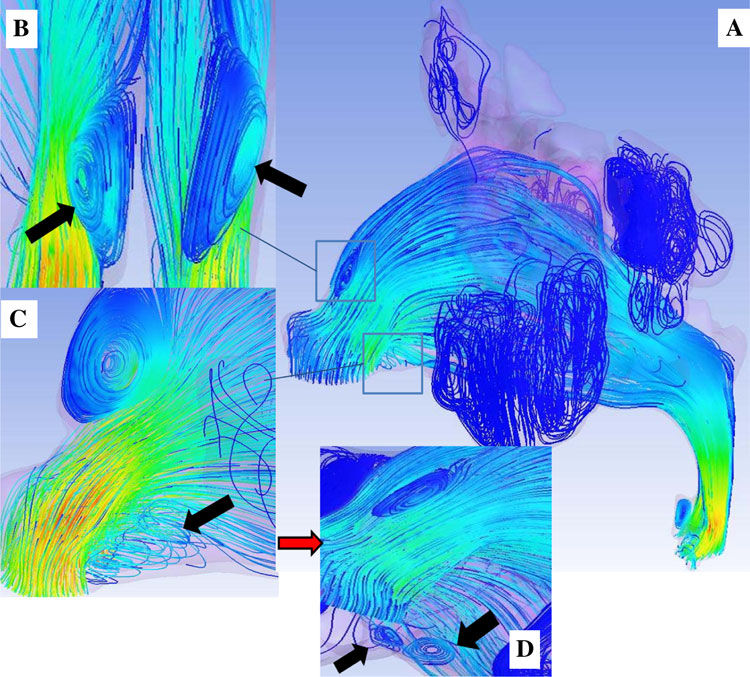
\includegraphics[width=0.5\textwidth]{chinstreams.png}
  \caption{Streamlines coloured by velocity from \cite{Tan2012}} \label{fig:chinstreams}
\centering
\end{figure}

\begin{figure}
  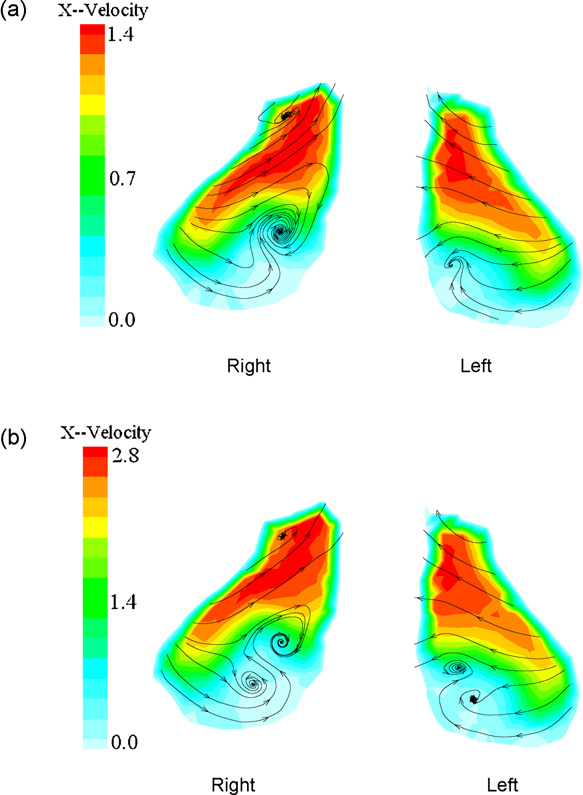
\includegraphics[width=0.5\textwidth]{wencont.png}
  \caption{Velocity contours at the nasal valve from \cite{Wen2008}} \label{fig:wencont}
\centering
\end{figure}
Airflow structures have been investigated and portrayed through a variety of both qualitative and quantitative methods. The earliest papers focused primarily on the pressure drop over the nostrils as measured with rhinomanometry\cite{Martin1981}. Modern technological innovation has facilitated the development of a range of techniques for both visualisation of airflows and the quantification of their various characteristics. In particular the range of data that can be obtained from numerical simulations is vast and detailed, and so the question of how to interpret it becomes particularly important.

One more commonly used visualisation method is the use of streamlines (shown in figure \ref{fig:chinstreams}). Streamlines, often coloured by velocity\cite{Wen2008, Zhu2011, Garcia2007}. These are useful for showing flow distribution as well as significant recirculation zones\cite{Lintermann2013, Xi2014}. Another commonly used method, shown in figure \ref{fig:wencont} is coronal cross sectional contours portraying velocity. These contours may or not include streamlines to help highlight the presence of vortices in the flow\cite{Wen2008}. Another method, presented in \cite{Lintermann2013} uses a $\Delta$ criterion to trace the vortices present in the flow structure. In \cite{Lintermann2013}, these are then coloured by variables related to turbulence and vorticity in order to provide a deeper insight in to the vortex structure and behaviour.

Quantitative methods for analysing and comparing air flow structures seem to be less standardised. Prior to the invention of modern imaging techniques, rhinologists relied on readings of cross sectional area and pressure from techniques such as rhinomanometry and acoustic rhinometry\cite{Doorly2008c}. The detailed flow information that can be extracted from CT scan models either experimentally or computationally opens up a much wider range of options in terms of quantitative analysis. Pressure is still often included as it is said to provide an insight in to the inspirational efficiency of the cavities\cite{Lintermann2013}. Pressure is often plotted as a function of flow rate in order to provide a point for validation by comparison with experimental set ups\cite{Wen2008, Inthavong2014}. In addition, it can be treated as a function of longitudinal position in order to gain an insight in to the relationship between the geometric variations and pressure drop\cite{Lintermann2013}. Another commonly measured variable is velocity distribution\cite{Keyhani1995, Zhu2011, Lintermann2013}. This can include cross sectional zone by zone analysis\cite{Keyhani1995, Zhu2011}, which has been suggested to be useful for the measurement of the efficacy of olfaction\cite{Zhu2011}, or by longitudinal sections\cite{Lintermann2013,Taylor2010} . Another commonly used quantitative measure is wall shear stress. Distributions are analysed longitudinally\cite{Wen2008} or around the cross sectional parameter of the relevant section of the nasal cavity\cite{Burgos2014}. These measurements have been shown to be significant for predicting heat and mass transfer characteristics\cite{Taylor2010}, and as such their longitudinal and parametric distributions are significant for understanding the distribution of such mechanisms.

\section{Demographic studies}
The previously investigated demographics include ethnicity\cite{Zhu2011}; disease\cite{Garcia2007}; and  age\cite{Xi2012}, which can then be subclassified into children\cite{Xi2012} and the elderly\cite{Lindemann2008}. Both of these have been investigated through both in vitro\cite{Weinhold2004} and in vivo\cite{Kalmovich2005, Edelstein1996, WhanKim2007, Lindemann2008} techniques. Child models have also been investigated computationally\cite{Xi2012}. The variations that have been observed in children's nasal airway functionality has been suggested to be linked to particle filtration ability \cite{Xi2012}. It seems plausible that this effect could be significant also in the case of elderly models. Cross sectional areas have been graphed as a function of radial position to compare the geometries of different models in many studies\cite{Xi2012, Zhu2011, Lindemann2008, Garcia2007}. Surface area has also been suggested to be significant metric in predicting flow behaviour (as surface area to volume ratios are expected to impact on the flow behaviour\cite{Xi2012, Garcia2007}). Resistance across the nasal cavity, measured as pressure drop, is also often used as a predictor of flow behaviour within the nasal cavity\cite{Edelstein1996, Lindemann2008, WhanKim2007}. As previously stated, streamlines are a commonly used method for visualising flow structures in nasal cavity models. They have as such been used in several instances to compare interdemographic variations in flow structure\cite{Xi2012, Garcia2007, Zhu2011}. Flow flux by saggital section across the turbinal region has also been used to identify variations in nasal functionality\cite{Zhu2011}. 


\section{Heat and vapour transfer}

Earlier investigations in to the heat and vapour transport characteristics of the nasal cavity used a straight pipe model as a simplification of the nasal cavity geometry\cite{Ingelstedt1961}. The first experiments involving real nasal cavity geometries were carried out in the 80s, using cast models taken from cadavers\cite{Nuckols1983}.

In vivo experiments into temperature variation across the nasal cavity have been done using various temperature measuring devices; modern experiments have tended towards using thermocouples because they are small and respond quickly\cite{Elad2008}. For measuring humidity in vitro, modern researchers have tended towards the use of capacitative humidity sensors\cite{Keck2000}. Detailed profiles of temperature and humidity throughout the nasal cavity have been presented by several past researchers\cite{Keck2000}.

CFD's have been used to simulate heat and vapour transfer in the nasal cavities with good accordance with experimental results\cite{Lindemann2004}. Early simulations investigating heat and vapour transfer used a steady state assumption for inflow conditions\cite{Naftali1998}. Later, the effect of the nasal cycle on temperature distributions was investigated, showing significant variations in the nasal temperature distributions throughout the nasal cycle\cite{Elad2006}.

Cross sectional temperature contours have been used to visualise the distribution of temperature throughout the nasal cavity; this provides a clear method visualising the distribution\cite{Naftali2005}. Saggital heat flux contours have also been used to similar effect\cite{Sullivan2013}. Heat flux, temperature, water flux and humidity have all been mapped as functions of position across the saggital axis in the nasal cavity\cite{Garcia2007, Sullivan2013, Yu2014}. The nasal valve has been noted from these observations to be a region of particular significance to heat and vapour transfer mechanisms\cite{Sullivan2013}. 




%\cite{Elad2008}
%
%in vitro studies - blood and mucous as transport agents for heat and moisture. Ingelstedt and Tolmalm, 1961, straight pipe simulation. Casting plastic Nuckols et al 1983, napthalene sublimation - Hanna and scherer, 1986. 
%
%In vivo studies - limited due to complexity of geometry, posterior Temperature 31-34 deg C, 90-95\%, Keck et al 2000 a, b. Variation of the nasal mucosa temperature, turbulence linked to higher heat flux values - Lindemann et al 2002. Temporal change in cavity flow - Eccles 2000; Hanif et al. 2000
%
%Computational - accurate 3d replica for predicting temperature distribution - Lindemann et al 2004, 2006, Pless et al 2004a, 
%
%Naftali et al. 2005, full 3d model for heat and vapour transfer in anatomical replica
%
%Wolf et al 2004 - psychometric charts used to calculate required heat and water to condition incoming air
%
%Naftali et al 2005 - varied inlet conditions show similar conditining capacity
%
%Kastl et al - impact of rhino-surgical interventions
%
%Influence of septal deviations - Pless et al. 2004b
%
%
%\cite{Garcia2007}
%
%Heat flux adjusted for evaporation as per (40)
%
%100\% RH at wall due to mucus
%
%vestibule zero water flux
%
%ambient air at 50\% RH, outflow at outlet
%
%mapped temperature across cavities, also relative humidity, water flux contours
%heat flux and water flux against length. Also as a function of height from nasal floor
%
%Tables of water flux per unit area
%
%flow partitioning
%
%pressure drop


\section{Literature gap}

To date, to the best of our knowledge, although some research has been carried out on the effects of aging on nasal airflow, CFDs have not been used to examine in depth the influence of age related variations in nasal cavity geometry on flow structure or heat and vapour transfer characteristics in older nasal caities. 

%\section{Particle filtration}
%
%

